\chapter{Evaluating the Algorithm on Real-World Data Sets}\label{ch:evaluation}
% !!! to fit on the page the text size in tables may be shorter + use a LOT of abbreviations
% WHAT DOES IT ALL MEAN? - jedes Ergebnis muss tiefgehend (tiefer als die anderen Paper) interpretiert werden!

In this chapter the modified SCM is experimentally evaluated on real-world data sets by conducting \(10 \times 10\) fold cross validations and other analyses,
as introduced in~\autoref{sec:evalMethods}.
Besides investigating on the algorithm's performance, the data sets themselves are also subject to intensive study,
in order to identify their underlying patterns and analyze crucial features and thresholds.
All of the following data sets are binary classification problems.
Their samples have no missing values and are all labeled.

First, two UCI data sets are analyzed in \autoref{sec:uci} to test the SCM on categorical and mixed type features.
Afterwards seven RNA sequencing data sets with high feature dimensions are evaluated in \autoref{sec:geneticData},
to demonstrate the numerical SCM and its applicability in biomedical contexts.
The hyper-parameters \(p\) and \(minConjSize\) will be individually adjusted on each
of these data sets.

\section{Methodology}\label{sec:evalMethods} % / Evaluation Techniques

% need test data
While it can be useful to run the SCM algorithm on all available samples, to see how a classification
rule based on this whole data set would look, the learning algorithm in general needs to be trained and tested on two
independent sample sets, in order for the testing results to be realistic.
However, since all data sets that are analyzed in this thesis only provide training data, but no
independent test data, it is best practice to delegate some of the training samples as test samples~\citep{kestler11}.

% cross validation
To minimize the influence of a more or less favorable selection of the training data subset,
a \(m \times n\) cross-validation, meaning a \(n\)-fold cross-validation, that is done on \(m\) different permutations of the data,
is usually employed for analyzing the performance of an SCM~\citep{muessel, kestler11}.
Within every \(n\)-fold cross-validation, the set of all samples is split into \(n\) groups of approximately equal sizes.
Over the course of the \(m\) iterations, every one of these groups is now once handled as the test group and
otherwise handled as of the training groups, ensuring that there are always \(n-1\) training groups and one test
group in every cycle.
The \(m \times n\) cross-validation finally results in \(m \cdot n\) independent models,
in this case in the form of classification rules.
Those models can then be analyzed as shown in \autoref{subsec:cvOutcomes}.

% cv performance + values for m and n
RAM space is in general no problem for cross-validation computations, as only
the current model, along with very few information about the previously computed models, need to be stored at a time.
However the algorithms runtime is usually crucial, as it is bounded in \(\mathcal{O}(l \cdot m \cdot n)\)
and not really reducible, since all models need to be computed independently.
Here \(l\) denotes the runtime of a single model computation on \(\frac{n-1}{n}\) of the available samples.
When evaluating an SCM, the number of chunks \(m\) and the number of permutations \(n\) are most commonly both set to 10~\citep{kestler11,lausser20}.
This is a good compromise between the high computation times when using high values for \(m\) and \(n\),
and the low utilization rates of samples for training the model, when using low values.

\begin{figure}
    \centering
    \begin{subfigure}{\textwidth}
        \centering
        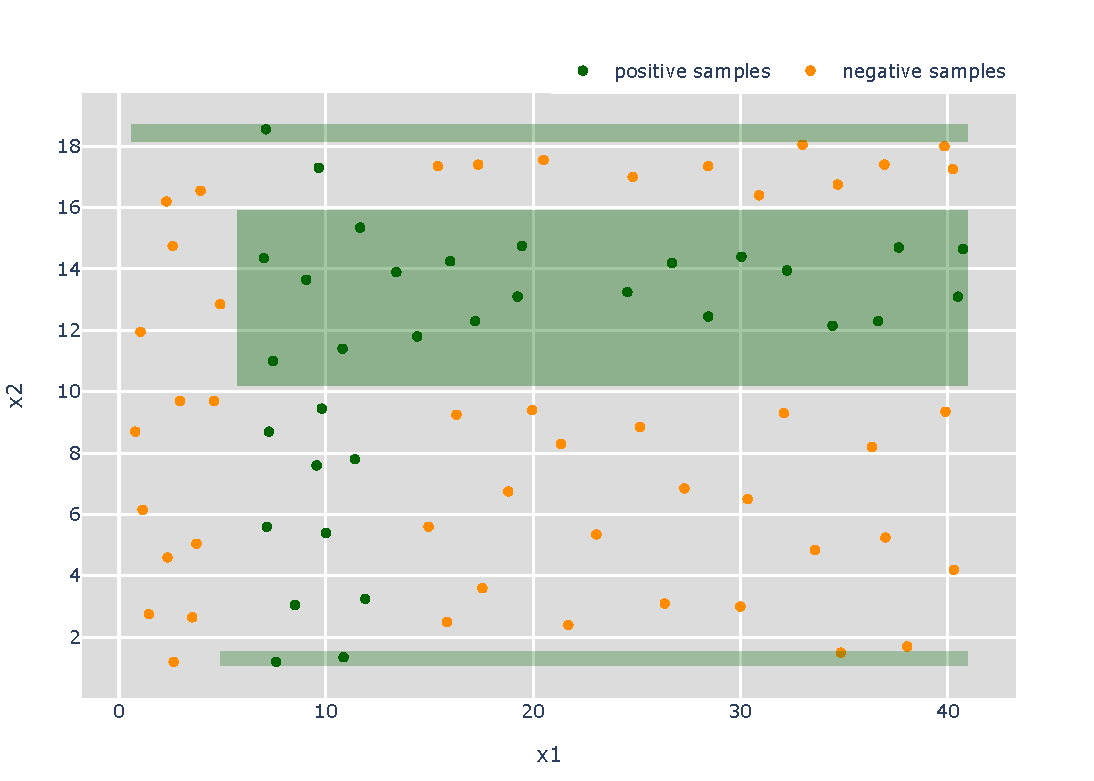
\includegraphics[width=0.85\columnwidth]{figures/cross_1.pdf}
        \caption{Training in the data set with unchanged labels.}
    \end{subfigure}
    \begin{subfigure}{\textwidth}
        \centering
        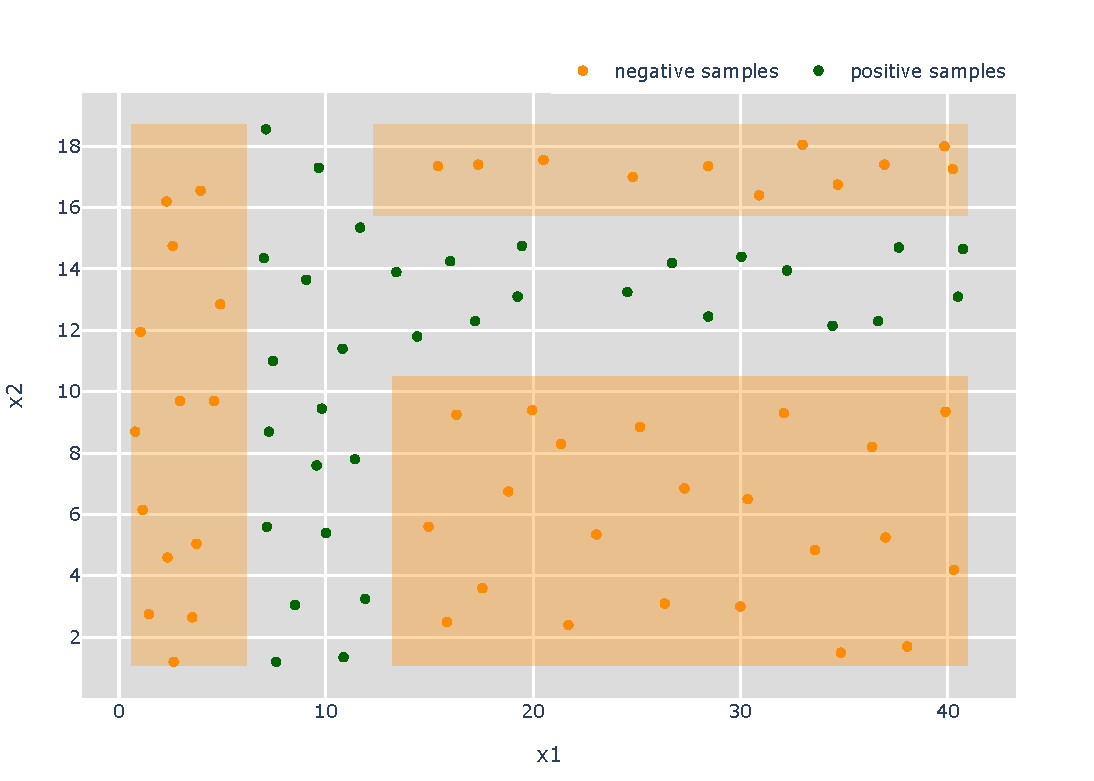
\includegraphics[width=0.85\columnwidth]{figures/cross_1_negated.pdf}
        \caption{Training on the data set with flipped labels.}
    \end{subfigure}
    \caption{Classification rule for an artificial data set with two orthogonal decision regions and its negative.
        Both models use a \(p = minConjSize = 1\).}\label{fig:crossNegative}
\end{figure}

% considering flipped labels
But after all, the \(m \times n\) cross-validation will produce more than 100 models,
as not only the decision rules for classifying samples as class 1, but also those for
classifying them as class 0, are considered, in order to compare the negated and the non-negated DNF and find the best possible models (see \autoref{julia:cv}).
This generally leads to an improved performance of the algorithm, as one context is often more favorable
than the other and therefore produces a better decision rule.
One example for such an improvement is displayed in \autoref{fig:crossNegative}.
In the context of nominal features, computing the decision rules for both classes is especially helpful, as
it often eliminates the need to implement an `\(\neq\)' operator as in `\texttt{IF x5 \(\neq\) green THEN class 1}', by instead using
the negated form `\texttt{IF x5 = green THEN class 0}'.
This negation can be done easily by executing the SCM algorithm twice: once with the unchanged data set \(S\)
and once with \(S\) having flipped labels.
Additionally it is important to set the hyper-parameter \(p\) as \(\sfrac{1}{p}\) and
switch the resulting sensitivity and specificity, when working with flipped labels,
in order to obtain the correct result for a class 0 classification.
After all, the process of finding the optimal model, or even models, can be quite complex, as there are multiple
objectives that the model should fulfill to the highest possible degree-
Yet \autoref{subsec:pareto} presents a highly efficient method to help with this selection.

%%%%%%%%%%%%%%%%%%%%%%%%%%%%%%%%%%%%%%%%%%%%%%%%%%%%%%%%%%%%%%%%%%%%%%%%%%%%%%%%%%%%%%%%%%%%
\subsection{Multi-Objective Model Selection Using Pareto Fronts}\label{subsec:pareto}

Whenever one needs to select a model that optimizes multiple different, often times even opposing, criteria, trade-offs are needed.
The SCM is especially known for the opposing objectives of its classification rules, as they
have to be accurate and compact at the same time.
Therefore a good strategy, to decide for a `good' classifier over a `bad' classifier, is strongly needed.
Traditionally those concurrent goals are assigned fixed weights, so the algorithm can form them into a
hierarchy and find the optimal model for this prioritization of goals, for example by using weighted sums~\citep{muessel}.
Yet, this mechanism has a very unflexible implementation and the weights need to be set in advance.

Another possibility is to use the approach of~\cite{muessel} of selecting all models which are pareto-optimal.
The algorithm works without any fixed weight relation of its objectives and allows all objectives to be treated separately.
A classifier \(b={b_1, b_2, \ldots}\) is pareto-optimal, if no classifier exists that dominates \(b\).
A classifier \(a={a_1, a_2, \ldots}\) would dominate \(b\), if and only if \(\forall i: a_i \geq b_i \land \exists j: a_i \ge b_i\).
In other words, \(b\) is pareto-optional, if and only if there is no other classifier that performs better than \(b\) in
all objectives (\(\nexists a: \forall i: a_i \geq b_i \land \exists j: a_i \ge b_i\))~\citep{muessel}.
This also means that two models with the same values regarding all goals, will always both be selected,
as long as they are not dominated by other models.
The user can then inspect all pareto optimal models and may, but does not have to, select one distinct winner by 
applying an implicit or explicit prioritization function to the objectives~\citep{muessel}.

In case of the SCM, the goal is to choose the best classification rule, regarding both performance aspects, like accuracy,
sensitivity and specificity, as well as compactness, with objectives like a minimizing the number of features and base classifiers.
In order not to make the process unnecessarily complex, I decided to choose only two of those metrics for my studies:
the accuracy, as the most comprehensive measure to describe a models performance, and the number
of features that are used in the decision rule, since the number of base classifiers is already pretty determined by \(sC\) and \(sD\).
Also the number of base classifiers might be subject to further minimization, while the number of features is certainly not.
This pareto front approach (see \autoref{julia:paretoFront}) is now used to determine
whether the model using flipped or un-flipped labels is better, or even both are interesting for
further investigation.

%%%%%%%%%%%%%%%%%%%%%%%%%%%%%%%%%%%%%%%%%%%%%%%%%%%%%%%%%%%%%%%%%%%%%%%%%%%%%%%%%%%%%%%%%%%%
\subsection{Analyzing the Insights Provided by Cross-Validation}\label{subsec:cvOutcomes}

In addition, pareto fronts can also be applied to the 100 or more models, that are the outcome of the
\(10 \times 10\) cross-validation, to filter out the most promising models.
However, one has to keep in mind, that all performance values, like the model's accuracy,
are only subject to \(\sfrac{1}{m} = \sfrac{1}{10}\) of all samples.
As the data sets that are discussed in this paper only contain a few dozen to a few hounded
samples, this share of test samples is so small, that the randomness and luck of
the cross-validation's chunk selection may heavily influence the results.
This leads to the fact that the pareto-optimal models here were actually only pareto-optimal on
a small fraction of the samples, yet cannot be tested on the other ones, as those samples were already used for training.
As a consequence, the set of pareto-optimal models has to be analyzed with high caution,
as the models from different cross-validation cycles are not really comparable to each other.

Therefore the focus is now shifted from working with optimums, to using the plot of the pareto fronts
for analyzing the scattering of the models in the two dimensional space of accuracy and complexity.
Relevant insights like the minimum accuracy of all models or the maximum number of features can be obtained easily here.
Also the percentage of models with accuracies above or below the accuracy baseline can be considered.
This baseline is defined as the fraction of samples in the largest class, to the total amount of samples.
A machine learning algorithm will always achieve an accuracy on the baseline, by simply classifying every sample to the larger class.
In case of heavily uneven classes, the algorithm then might even have a seemingly good accuracy,
however per definition it only learned something valuable, if it is able to outperform the baseline on unseen test data.
However one needs to keep in mind, that this two dimensional plot is constructed in such a way,
that one point in the space may stand for only one or a whole set of models.
Therefore the true distributions of the models cannot be derived from the plots and additional tools to analyze averages are needed.

% Averages
Additionally measurements of the mean characteristics of the models, like the average number of features,
base classifiers or conjunctions per rule, as well as the average accuracy, specificity and sensitivity can be very helpful for certain analysis.
Those values may usually be considered without precautions, as the influences of randomness are evened out by working with medians.
The average accuracy furthermore equals \(1 - \text{cross-validation error}\), where the
cross validation error estimates the generalization error~\citep{muessel}.
To put the number of features, that are used within a classifier, into a context,
the feature compression rate \(1-\frac{|\text{`features in rule'}|}{|\text{`all features'}|}\) might be helpful.
It can be interpreted as the percentage of features that can be reduced by using this
classifier, instead of dealing with the original data set.
Most of the results, including those means, are rounded to two or three decimal digits.
However, this is always done carefully in such a way, that it does not effect the results's interpretations, but only improves the readability a bit.

Another way to represent averages is by using histograms that display what percentage of models share a certain characteristic.
A histogram about the most used features showcases important information about the importance of each feature,
while histograms about the most used base classifiers, both, for base classifiers that contribute to a classification
of the sample as class 0 and as class 1, reveal the main structures within the class distribution.
This separate study of class 0 and class 1 base classifiers is needed, as they have opposing objectives.
In order to make those histograms as informative as possible without flooding the viewer with useless
information, only those base classifiers and features are displayed, that occur in at least 20\% of all
models and can therefore be considered as common.